\documentclass[a4paper,12pt,oneside]{report}
\usepackage{enumitem}
\usepackage{wrapfig}

\usepackage{amsmath}
\setdescription{leftmargin=\parindent,labelindent=\parindent}
\usepackage[lmargin=1.5cm, rmargin=1.5cm,tmargin=2.50cm,bmargin=4cm]{geometry}
\usepackage{array}
\usepackage[Bjarne]{fncychap}
\usepackage{amsrefs} 
%\usepackage[utf8]{vietnam}
\renewcommand{\thesection}{\arabic{section}}
\usepackage{graphicx}
\usepackage{listings}
\setlength{\textwidth}{16cm} \setlength{\textheight}{22cm}
\setlength{\oddsidemargin}{0.5cm} %\setlength{\topmargin}{2.5cm}
%\setlength{\botmar}{length}
\setlength{\evensidemargin}{0.5cm} %\setlength{\topmargin}{0cm}
\usepackage{hyperref}
\usepackage{fancyhdr}
\pagestyle{fancy}
\lhead{\textsc{Semester Project Fall 2015}}
\rhead{{\textsc{EURECOM Institute}}}
\renewcommand{\headrulewidth}{0.4pt}
\renewcommand{\footrulewidth}{0.4pt}
\usepackage{graphicx}
\usepackage{caption}
\usepackage{subcaption}
\setcounter{secnumdepth}{3}
\usepackage{epstopdf}
\usepackage[acronym]{glossaries}
\setcounter{tocdepth}{3}
\newcommand{\mychapter}[2]{
    \setcounter{chapter}{#1}
    \setcounter{section}{0}
    \chapter*{#2}
    \addcontentsline{toc}{chapter}{#2}
}

\makeglossaries
\usepackage{color}
\setcounter{secnumdepth}{4}
\definecolor{mygreen}{rgb}{0,0.6,0}
\definecolor{mygray}{rgb}{0.5,0.5,0.5}
\definecolor{mymauve}{rgb}{0.58,0,0.82}

\lstset{ %
  backgroundcolor=\color{white},   % choose the background color; you must add \usepackage{color} or \usepackage{xcolor}
  basicstyle=\footnotesize,        % the size of the fonts that are used for the code
  breakatwhitespace=false,         % sets if automatic breaks should only happen at whitespace
  breaklines=true,                 % sets automatic line breaking
  captionpos=b,                    % sets the caption-position to bottom
  commentstyle=\color{mygreen},    % comment style
  deletekeywords={...},            % if you want to delete keywords from the given language
  escapeinside={\%*}{*)},          % if you want to add LaTeX within your code
  extendedchars=true,              % lets you use non-ASCII characters; for 8-bits encodings only, does not work with UTF-8
  frame=single,                    % adds a frame around the code
  keepspaces=true,                 % keeps spaces in text, useful for keeping indentation of code (possibly needs columns=flexible)
  keywordstyle=\color{blue},       % keyword style
  language=Octave,                 % the language of the code
  otherkeywords={*,...},            % if you want to add more keywords to the set
  numbers=left,                    % where to put the line-numbers; possible values are (none, left, right)
  numbersep=5pt,                   % how far the line-numbers are from the code
  numberstyle=\tiny\color{mygray}, % the style that is used for the line-numbers
  rulecolor=\color{black},         % if not set, the frame-color may be changed on line-breaks within not-black text (e.g. comments (green here))
  showspaces=false,                % show spaces everywhere adding particular underscores; it overrides 'showstringspaces'
  showstringspaces=false,          % underline spaces within strings only
  showtabs=false,                  % show tabs within strings adding particular underscores
  stepnumber=2,                    % the step between two line-numbers. If it's 1, each line will be numbered
  stringstyle=\color{mymauve},     % string literal style
  tabsize=2,                       % sets default tabsize to 2 spaces
  title=\lstname                   % show the filename of files included with \lstinputlisting; also try caption instead of title
}




\begin{document}

\begin{titlepage}

\newcommand{\HRule}{\rule{\linewidth}{0.5mm}} % Defines a new command for the horizontal lines, change thickness here

\center % Center everything on the page
 
%----------------------------------------------------------------------------------------
%	HEADING SECTIONS
%----------------------------------------------------------------------------------------

\textsc{ 
	Graduate School and Research Center In communication Systems} % Name of your university/college
\begin{center}

\includegraphics[scale=0.5]{eurecom.png}
\end{center}

\textsc{\large Semester Project Report}\\[2cm] % Minor heading such as course title

%----------------------------------------------------------------------------------------
%	TITLE SECTION
%----------------------------------------------------------------------------------------

\HRule \\[0.4cm]
{ \Large \bfseries Attack Crawler for Modern Networked Systems}\\[0.4cm] % Title of your document
\HRule \\[1.5cm]


 
%----------------------------------------------------------------------------------------
%	AUTHOR SECTION
%----------------------------------------------------------------------------------------

\begin{minipage}{0.57\textwidth}
\begin{flushleft} 
\emph{Group}\\
\quad \textbf{TRUONG Quang-Huy}\\
\quad \textbf{VO Huynh-Dan}\\


\end{flushleft}
\end{minipage}
~
\begin{minipage}{0.4\textwidth}
%\begin{flushright} 
%\emph{RESPONSABLES:} \\
%Prof. \textbf{Christian Bonnet} % Supervisor's Name
%\end{flushright}
\begin{flushright} 
\emph{Supervisors:} \\
\textbf{Yves Roudier} \\
\textbf{Ludovic Apvrille} \\

\end{flushright}

\end{minipage}\\[3cm]

% If you don't want a supervisor, uncomment the two lines below and remove the section above
%\Large \emph{Author:}\\
%John \textsc{Smith}\\[3cm] % Your name

%----------------------------------------------------------------------------------------
%	DATE SECTION
%----------------------------------------------------------------------------------------

{ Biot, \today}\\[3cm] % Date, change the \today to a set date if you want to be precise

%----------------------------------------------------------------------------------------
%	LOGO SECTION
%----------------------------------------------------------------------------------------

%\includegraphics{Logo}\\[1cm] % Include a department/university logo - this will require the graphicx package
 
%----------------------------------------------------------------------------------------

\vfill % Fill the rest of the page with whitespace

\end{titlepage}
\linespread{1.3}
\pagenumbering{roman}

%\chapter*{Acknowledgement}

%In performing our assignment, we had to take the help and guideline of some respected persons, who deserve our greatest gratitude. The completion of this assignment gives us much Pleasure. We would like to show our gratitude Mr. PUZIO Pasquale, for giving us a good guideline for assignment throughout numerous consultations. We would also like to expand our deepest gratitude to all those who have directly and indirectly guided us in writing this assignment.

%In addition, a thank you to Professor MOLVA Refik, who introduced us to the Methodology of work, and whose passion for the “underlying structures” had lasting effect. 

%Many people, especially our classmates and team members itself, have made valuable comment suggestions on this proposal which gave us an inspiration to improve our assignment. We thank all the people for their help directly and indirectly to complete our assignment.
%\begin{center}
%--------------------oOo--------------------
%\end{center}

%\begin{center}
%\textbf{Eurecom group}
%\end{center}
%\chapter*{Abstract}

%This report demonstrates a simple mechanism protocol, proposed by Mr. PUZIO Pasquale, for deduplicating data of cloud storage in client side which reduces the risk of data leakage from \acrfull{csp}. The mechanism bases on differences between the popular data which have a low sercurity level and un-popular which have schematically security. Besides, the mechanism also has some advantages in efficiency and security level when comparing with other mechanisms. 
%=========================================================
% table of contents, table of figures, table of tables
\tableofcontents
\printglossary
\cleardoublepage
\setcounter{page}{1}
\pagenumbering{arabic}
\setlength{\parindent}{4em}

%\thispagestyle{empty}

%\listoffigures

%\listoftables

\newpage

\pagenumbering{arabic}

% ========================================
% abbreviation and glossary






%\newacronym{api}{API}{Application Programming Interface }

%%% The glossary entry the acronym links to   
\newacronym{pir}{PIR}{Private Information Retrieval}
\newacronym{pow}{PoW}{Proof of Ownership}

\newacronym{idx}{IDX}{Index Service}
\newacronym{phf}{PHF}{Perfect Hash Function}
\newacronym{cof}{COF}{Confirmation of a file}
\newacronym{lri}{LRI}{learn-the-remain-information}
\newacronym{ce}{CE}{Convergent Encryption}
\newacronym{cd}{CD}{compact disk}
\newacronym{sv}{S}{secret value}
\newacronym{ks}{KS}{key server}
\newacronym{csp}{CSP}{Cloud Storage Provider}
\newglossaryentry{apig}{name={API},
	description={An Application Programming Interface (API) is a particular set
		of rules and specifications that a software program can follow to access and
		make use of the services and resources provided by another particular software
		program that implements that API}}

%%% define the acronym and use the see= option
\newglossaryentry{api}{type=\acronymtype, name={API}, description={Application
		Programming Interface}, first={Application
		Programming Interface (API)\glsadd{apig}}, see=[Glossary:]{apig}}


%========================================

\mychapter{1}{Introduction} 
\section{Project Description}
	Numerous large scale attacks on networked systems have been conducted in recent years, like
the Zeus/Zitmo attack on mobile banking systems, the Stuxnet and Havex malware that were
discovered on SCADA systems, or even the unlikely botnet infection of smart fridges.
Unfortunately, the study and analysis of those attacks is quite complex and requires gathering
information from very diverse sources. In addition, documenting and disseminating the knowledge
acquired in this process is often a largely manual process in which a lot of technical details get
lost and which is difficult to keep up to date with new vulnerabilities.
The objective of this project is to evaluate which relevant information can be automatically
extracted from Internet sources to better detect, understand, and model such persistent threats.
In particular this project will develop a crawler for assembling all such data and to integrate them
into TTool, a modeling environment featuring the SysML-Sec framework\cite{stuxnet1} defined by EURECOM
and Telecom ParisTech.

\section{Work Description}
Our works in this project include:
\begin{itemize}
\item We are provided with a few models of attacks captured manually with TTool and practice modeling with an additional known attack Stuxnet attack.
\item We implement a modeling assistant.
\end{itemize}

\mychapter{2}{Modeling an attack}
	\section{Introduce Stuxnet}
		
		Stuxnet\cite{stuxnet2} is a computer worm discovered in June 2010. It was designed to attack industrial control systems or set of similar systems. The goal of the attack is to reprogram industrial control systems by modifying code on programmable logic controllers (PLCs). The whole process of attack is deeply hided and covered in the system. However, the purpose and the identity of attackers are unknown, yet they are skilled and well resourced; this wasn't something that was put together in a short period of time. Four zero-day vulnerabilities are exploited in order to achieve this goal.
		
	\section{Model Stuxnet's attack in TTool}	
	To understand clearly about Stuxnet, we describe the attack of Stuxnet as SysML-Sec attack models by using TTool.
	The General model is used for a general understanding of Stuxnet. Furthermore, important components are also described in detail in distinct models such as Execute\_Stuxnet, Inject\_To\_Project\_Files, and Modify\_PLCs.
	\subsubsection{Diagram's Components}
	\begin{itemize}
		\item Tree Diagram: a diagram describles all possible attacks on
the system with the interconnetion between attacks and blocks. 
		\item Block: is an actor involving in the attack case.
		\item Attack: a malicious action performed in a block. There are two kinds attack: normal and root attack. Root attack is a final target in an Attack Tree 
		\item Contraint: relations between attacks such as:  OR, AND, SEQUENCE, BEFORE, AFTER.
	\end{itemize}
	\subsubsection{Stuxnet Operation}
	In the Gerneral model \ref{pic:gsmodel} , we can easily and quickly understand the purpose and procedure of Stuxnet. In particular, the final target of it is to modify PLCS in Siemens supervisory control and data acquisition (SCADA) system. To achieve this, Stuxnet attacks the system step by step. It takes advantages of zero-day vulnerabilities to propagate itself. In addition, it also uses rootkits, advanced techniques to hide itself from users and anti-virus software, on both Windows and the control computers it targets. Then, Stuxnet install itself and infects Siemen SIMATIC Step7 sofware.
	\begin{figure}[hb]
	 \centering
	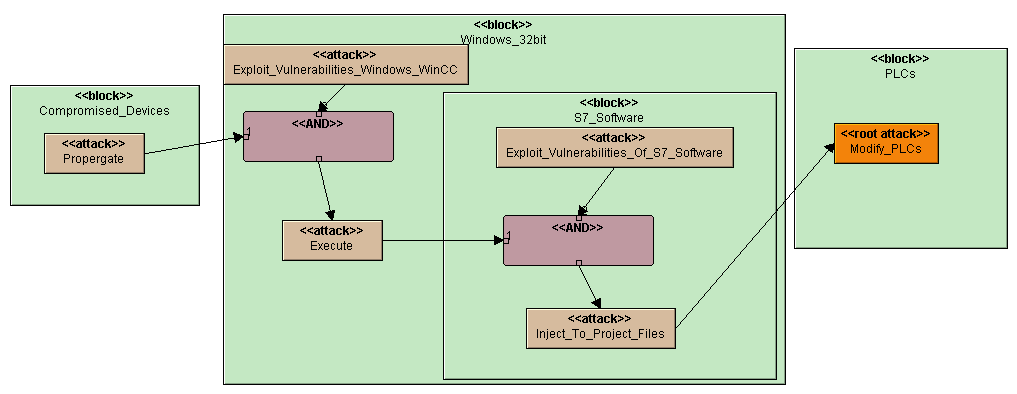
\includegraphics[scale=0.45]{General_Stuxnet.png}\par
	\caption{General Stuxnet diagram}
	\label{pic:gsmodel}
	\end{figure}
	Stuxnet spreads rapidly, but it also has mechanism to limit its spread. As illustrated in \ref{pic:esmodel}, Stuxnet employs numerous methods to spread itself\cite{stuxnet3}:
	\begin{itemize}
	\item Via USB flash drives, Stuxnet can use Windows LNK vulnerability or autorun.file vulnerability to spread. For LNK exploit, when .LNK files are displayed in windows explorer and the icon for a .LNK file is loaded. The malicious .LNK files contain an exploit code that will be excuted automatically . For autorun.inf file,  Stuxnet inserts the malicious code into the file, along with with commands to excute this code when autorun feature is enable.
	\item Via Print Spooler zero-day vulnerability, this vulnerability allows Stuxnet to copy itself on remote computers, then execute the copy to infect targets. 
	\item Via network shares vulnerability, the worm distributes itself over the network through shared folders by using either a scheduled job, and Windows Management Instrumentation. It copies itself on anyshares on remote computers, and schedule a task to execute it.
	\item Via WinCC. Stuxnet sends malicious SQL code to a system running with WinCC database using a hardcoded password that allows Stuxnet to be transfered to that system and excutes itself.
	\item Via Microsoft Server Message Block (SMB) vulnerability, Stuxnet sends a malformed path over SMB to excute arbitrary code on the remote system in order to propagate itself.\\\\
	\begin{figure}[hb]
	 \centering
	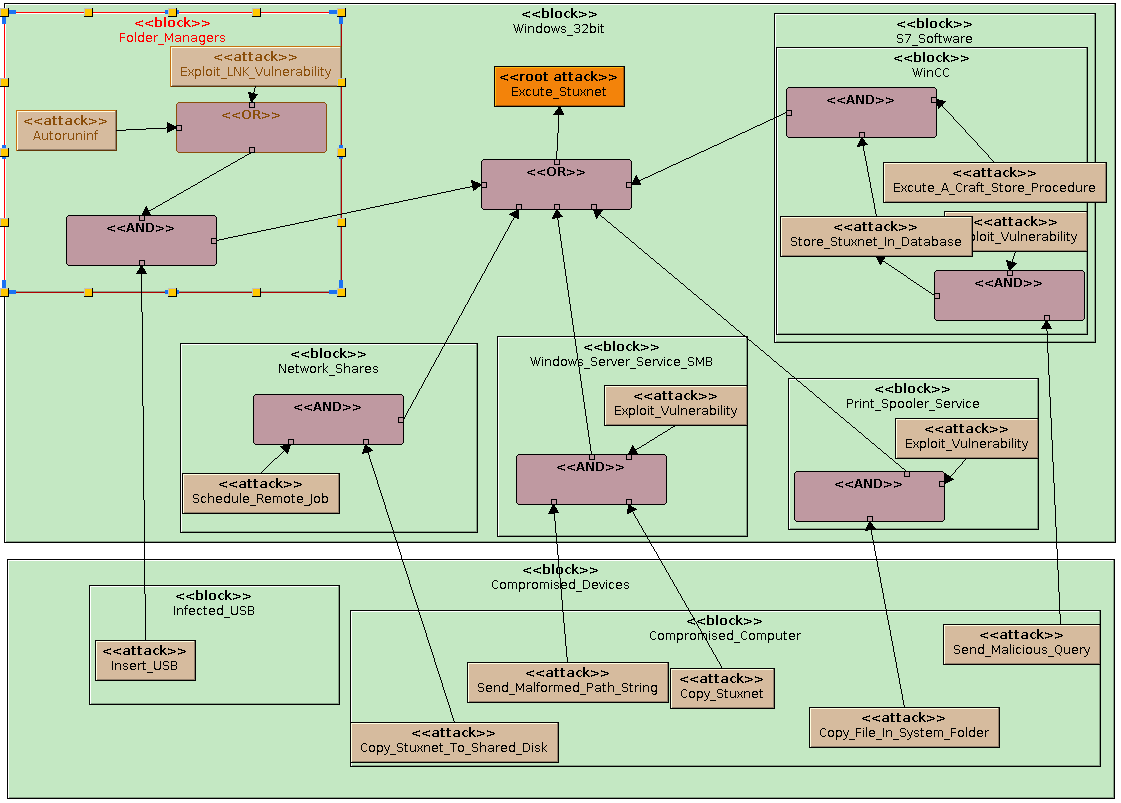
\includegraphics[scale=0.40]{Execute_Stuxnet.png}				\caption{Execute Stuxnet diagram}
	\label{pic:esmodel}
	\end{figure}
After being executed, Stuxnet will try to attain the root privilege by  using  one of two zero-day escalation of privilege attacks which are Win32k.sys and Task Scheduler Escalattion vulnerabilities. Together with advanced bypass antivirus techniques, Stuxnet tries to inject payload into the target process which infects directly to Step7 project files, and finally infects the project folder \ref{pic:ismodel}.\\
	\begin{figure}[hb]
	\centering
	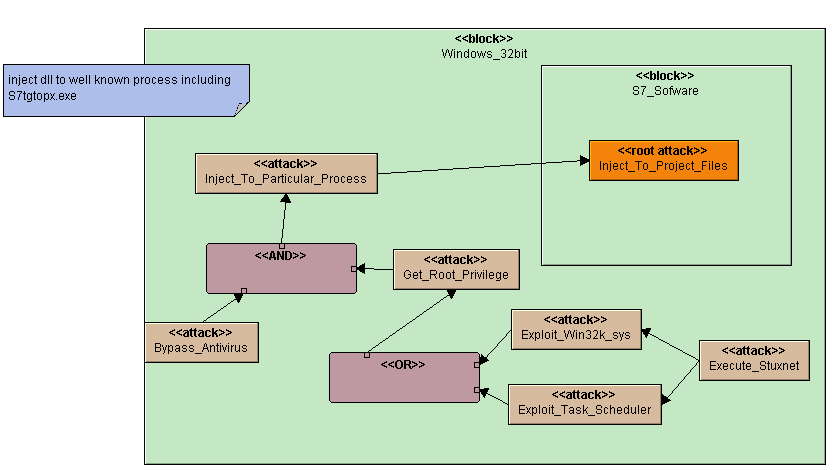
\includegraphics[scale=0.6]{Install_Stuxnet.png}
	\caption{Inject Stuxnet to project files diagram}
	\label{pic:ismodel}
	\end{figure}
Once Stuxnet is executed, it will overwrite the original DLL file named \textit{s7otbxdx.dll} that allows Stuxnet intercept any call between PLCs and Step7 Software \ref{pic:mpmodel}. Eventually, Stuxnet will be able to perform actions: Monitor PLC blocks being written to and read from the PLC; Inserting and replacing or infecting blocks; And Hiding injected code.
	\begin{figure}[hb]
	 \centering
	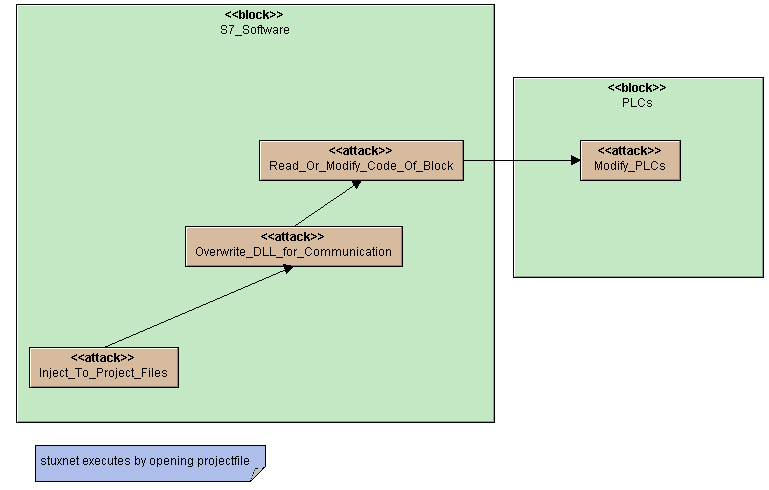
\includegraphics[scale=0.70]{Modify_PLCs.png}
	\caption{Modify PLCs diagram}
	\label{pic:mpmodel}
	\end{figure}
	\end{itemize}
\mychapter{3}{TTool search module}
		\section{Requirement}
Currently, TTool has a function to find components inside a SysML-Sec model according to an input string provided by users. The main purpose is to support for locating components in the model. There is a concern that users would like to inquire more information about graph components. In particular, it could be the technical detail of components, the other relationship between components and the variant of the component. However, this piece of information could not be embedded in these components. \\\\
The approach in this part of the project is to extract the data from outside TTool; Especially, on the internet and databases. From the internet perspective, thanks to search engine such as Google and Google Scholar, the finding of relevant information can be performed by an URL to these services. Another way of retrieving information is to access databases, the other part of this project. Therefore, main requirements in this part includes:
		\begin{itemize}
			\item  Implementing a GUI allowing users to perform extended search from outside resources by strings and following options.
			\item  Retrieving results from the internet, namely Google and Google Scholar.
			\item Designing and implementing a protocol to communicate with the database in order to get information and display to users.
		\end{itemize}
		\section{Environment}
		As an extention for Ttool's User Interface, this part of project involes directy to source code of TTool, which is competable with Java 7.\\\\
		There is an external library named JSoup\cite{jsoup} is taken as advantages in order to manipulate the request, response to Search Engine, and parse the HTML-format response. JSoup is an open source project distributed under the liberal MIT license. It can be found at http://jsoup.org/. Jsoup jar jsoup-1.8.1.jar is put in ./bin directory. Then, the Makefile is modified to ensure TTool will load the library.
\begin{lstlisting}[language=bash]
	basic:
	$(JAVAC) $(SOURCEPATH) $(TTOOL_SRC) $(CLASSPATH) $(TTOOL_BIN)/jsoup-1.8.1.jar $(TTOOL_SRC)/*.java	
		\end{lstlisting}
		\section{Graphic interface}
		As requirements, users desire to retrieve more information which either directly or indirectly relevant to elements in a working model. The task is to create an interface allowing users to interact with search engine.\\\\
		The graphic interface needs keywords from users as inputs which are obtained through several ways. In specific, there are two techniques to input keywords. Users can input them directly or simply, keywords can be obtained from component names.\\\\
		For the convenience, users have four options to compose a desired keyword by:
		\begin{itemize}
			\item Typing keywords into the search field on the menu bar of TTool.
			\item Pressing Ctrl and left-click on a component to get a name as keyword.
			\item Pressing Ctrl and left-click on components consequently, then right-click on the model and select option "External Search". The list of names of selected components will be combined as a keyword.
			\item Pressing Ctrl - Alt and left-click on a component. The form will be displayed with the name of selected component.
			\item When the form is shown, users can modify a keyword by pressing Ctrl and left click on that component. 
			\item In addition, users modify a keyword directly on the search field of the dialog
		\end{itemize}
		To open the External search dialog, users can perform those actions:
		\begin {itemize}
		\item From the main menu Tool $\rightarrow$ External Search\par
		\begin{center}
		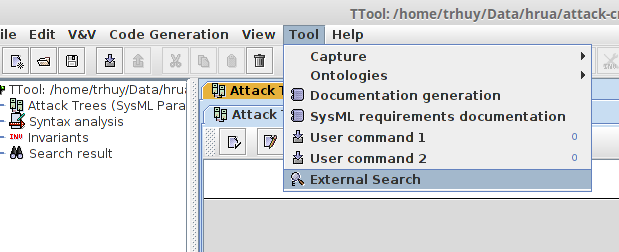
\includegraphics[scale=0.6]{mainmenu_crop.png}
		\end{center}
		\item From  working graph, through the context menu ( Right click  $\rightarrow$ External Search ) \\\\
		\begin{center}
		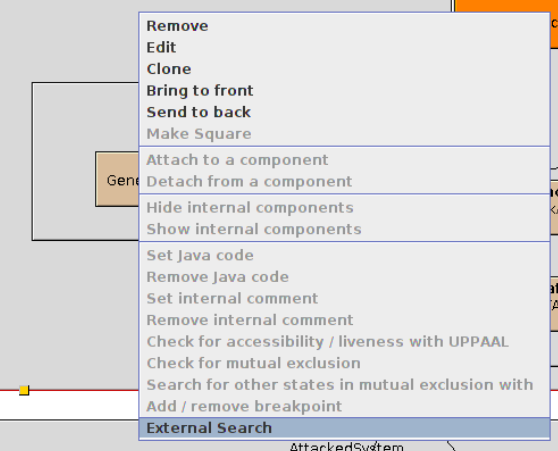
\includegraphics[scale=0.5]{contextmenu_crop.png}
		\end{center}
		\item From the menu bar, through the icon External Search.\\\\
		\begin{center}
		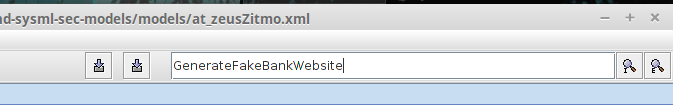
\includegraphics[scale=0.6]{menubar.png}
		\end{center}
		\item  Pressing Ctrl-Alt and left-click on a component. The form are displayed with the name of selected component.
		
		\end{itemize}
		On the dialog, a query is constructed by collecting the keyword, options, target data resources. As well as, there are tables and text fields to represent searching results. \\\\
		\begin{center}
		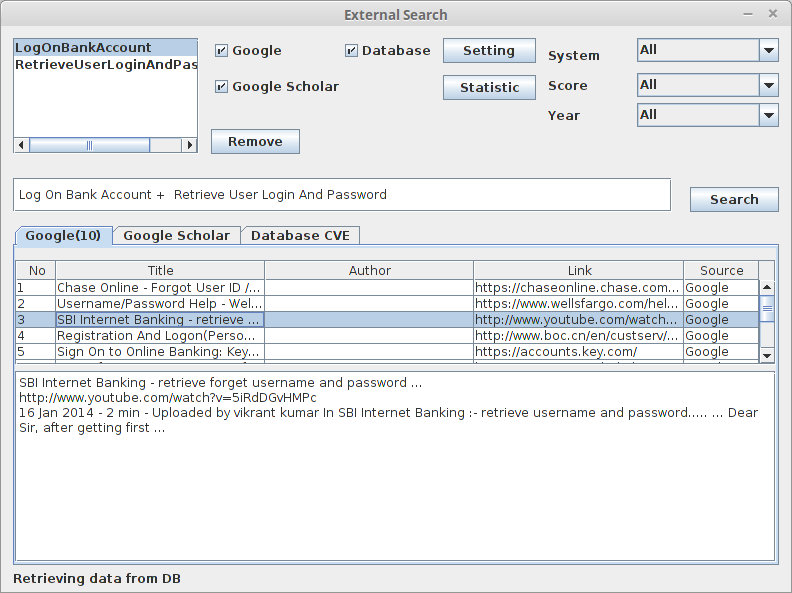
\includegraphics[scale=0.5]{ExternalSearch.png}
		\end{center}
		To optimize the keyword for searching, name of selected components will automatically split into distinct words.\\\\
		For each target data resource such as Google, Google Scholar, and Database, there are tabs to display those results separately.\\\\
		The related source code for the External Search GUI :
		\begin {itemize}
			\item \textit{./src/ui/window/JDialogSearchBox.java} : This is the main implimentation of GUI for Searching Dialog. 
			\item \textit{./src/ui/TDiagramPanel.java} : Menu context is added into the option for External Search.
			\item \textit{./src/ui/TDiagramMouseManager.java} : A few lines of code for caching the event of mouse when clicking on components with special keys ( Ctrl, Alt) 
			\item \textit{./src/ui/MainGUI.java} : The instance of JDialogSearchBox belongs to MainGUI which allows the search function can be accessed by every context of TTool. 
			An added code supports to reuse the search field in menu bar for both Internal Search and External Search. It also allows to open a External Search Dialog by a button beside the search field. 
			\item \textit{./src/ui/TGUIAction.java} : register  new actions for Internal and External, including icons and description.
			
		\end {itemize}
		
		\section{Internet Search}
		The goal of this function is to parse a returned searching result in HTML format from Google search engine for specific string queries.
		For Google and Google Scholar, the query string is sent to servers by GET method. Two parameters applied here are "\&q=" and "\&num=" to supply the query and number of result for that query, respectively.\\\\
		The URLs are:\par
		\textit{http://www.google.com/search?hl=en\&q=\textless string \textgreater\&num= \textless number \textgreater}\par
		\textit{http://scholar.google.com/scholar?ht=en\&q=\textless string \textgreater\&num= \textless number \textgreater}\\\\
		Thanks to JSoup library, DOM objects in HTML content are parsed and displayed in GUI.
		Structure of HTML content from Google with selector syntax of CSS includes:\par
		\begin {itemize}
		\item List of search results : \textit{li.g}\par
		\item Each search results has:
		\begin {itemize}
			\item Link: \textit{a} tag with \textit{href}
			\item Description: the element with \textit{span.st}
		\end{itemize}
		\end{itemize}
		Structure of HTML content from Google Scholar with selector syntax of CSS:\par
		\begin{itemize}
		\item List of search results : \textit{div.gs\_ri} \par
		\item Each search results has:
		\begin {itemize}
			\item Link: the element with \textit{h3.gs\_rt \textgreater a} 
			\item Description: the element with \textit{div.gs\_rs}
			\item Author: the element with \textit{div.gs\_a}
			\item Cites: the element with \textit{div.gs\_fl \textgreater a}
		\end{itemize}
		\end{itemize}
		The related source code for the Google Search
		\begin {itemize}
			\item ./src/myutil/GoogleSearch.java: a class represents for an article in result of google search. It has two functions to fetch data from Google and Google Scholar. \ref{fGoogleSearch}
\begin{table}[h]
\centering

\begin{tabular}{lll}
\hline
\multicolumn{1}{|l|}{\bf Functions}              & \multicolumn{1}{l|}{\bf Descriptions}                                                                                                                               & \multicolumn{1}{l|}{\bf Returned Type}           \\ \hline
\multicolumn{1}{|l|}{getGoogleResult}        & \multicolumn{1}{l|}{\begin{tabular}[c]{@{}l@{}}execute the search query to\\ Google, the result is stored in\\ a list of  GoogleSeach objects\end{tabular}}        & \multicolumn{1}{l|}{ArrayList\textless GoogleSearch\textgreater} \\ \hline
\multicolumn{1}{|l|}{getGoogleScholarResult} & \multicolumn{1}{l|}{\begin{tabular}[c]{@{}l@{}}execute the search query to\\ GoogleScholar, the result is stored \\in a list of GoogleSeach objects\end{tabular}} & \multicolumn{1}{l|}{ArrayList\textless GoogleSearch\textgreater} \\ \hline                                    
\end{tabular}
\caption{Functions of GoogleSearch class}
\label{fGoogleSearch}
\end{table} 
			\item ./src/myutil/CheckConnection.java: functions to check the connection to servers.\ref{checkConnection}
			
\begin{table}[h]
\centering
\begin{tabular}{|l|l|l|}
\hline
{\bf Functions} & {\bf Descriptions} & {\bf Returned Type} \\ \hline
checkInternetConnection & \begin{tabular}[c]{@{}l@{}}check if client can connect to\\  default address and url.\end{tabular} & Boolean \\ \hline
checkConnectionWithAddr & \begin{tabular}[c]{@{}l@{}}check if client can connect to\\  a specific address.\end{tabular} & Boolean \\ \hline
\end{tabular}
\caption{Functions of CheckConnection class}
\label{checkConnection}
\end{table}

\end {itemize}
		\section{Database Search}
		Similarly, this feature connects to a database created by Crawler in order to extract relevant information. Furthermore, users also have general view of vulnerabilities in the database through visualization. 
		
\subsection{Protocol}
	\subsubsection{Objective}
	The aim of the protocol is to connect TTool and Web crawler. In particular, TTool users can retrieve relevant information from databases that needs help from Web crawler, so they need to unify a protocol to exchange information. In addition, we also need to secure the information. 
	
	\subsubsection{Design}
	The protocol is divided into two directions, client side (TTool users) and a multithreaded server side (Web crawler). A new class named “Message” which is a unified structure used to supply functions for both clients and server. In addition, the protocol implements "Serializable" in order to exchange "Message" between clients and server.\\\\
	Because of the confidentiality, data integrity of the message, and client-server authentication , SSLSocket technique which is a cryptographic protocol for secure Internet data transmission is implemented to make sure these properties. Exchanged messages between clients and server need to be secured. We want to make sure that clients can talk to the right server and vice versa. Furthermore, nobody has the permission to modify messages while they are being exchanged.
	
	\begin {itemize}
	\item First of all, GUI of TTool allows users to select and choose information they need to retrieve from the database. 
	\begin{center}
	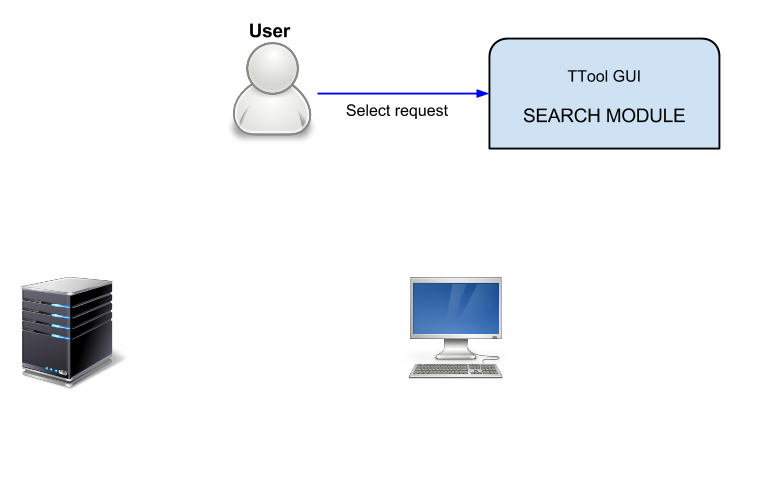
\includegraphics[scale=0.5]{Protocol1.png}\par
	\end{center}
	
	\item Secondly, information is sent to client side which then is created and stored in a request message by client and sent to the server. 
	\begin{center}
	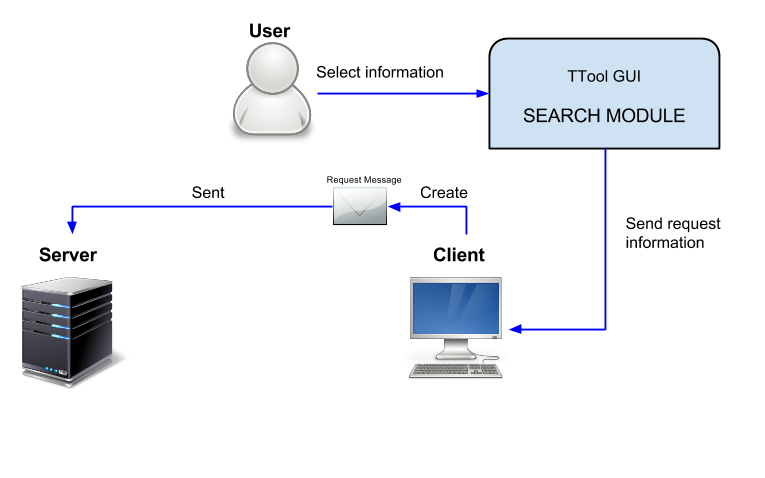
\includegraphics[scale=0.5]{Protocol2.png}\par
	\end{center}
		
	\item Next, the server is responsible for analyzing the request message and retrieve, search for relevant information which matches with client requirements. 

	\begin{center}
	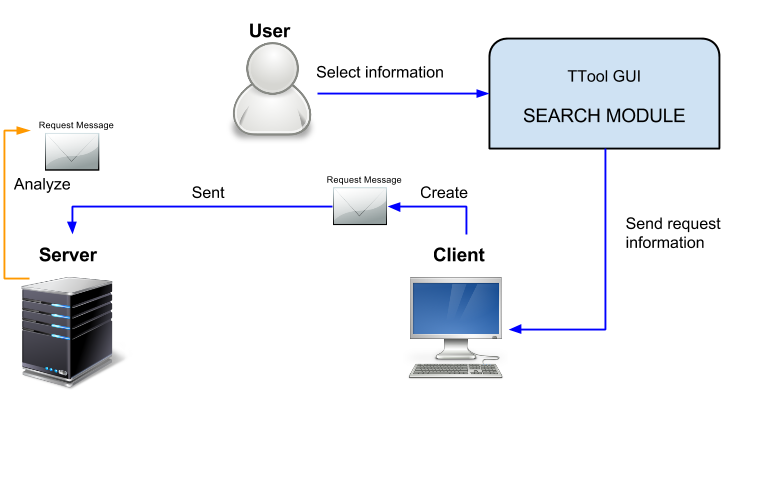
\includegraphics[scale=0.5]{Protocol3.png}\par
	\end{center}
	
	\item In the next phase, relevant information is stored in an answer message and sent back to the client. 

	\begin{center}
	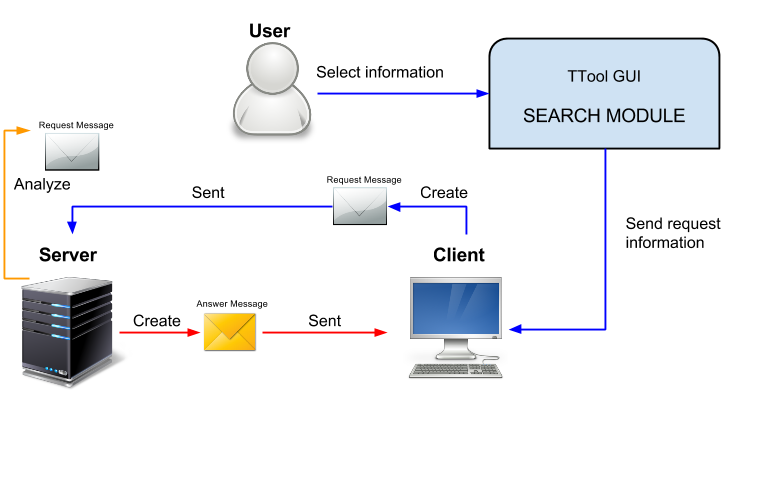
\includegraphics[scale=0.5]{Protocol4.png}\par
	\end{center}
		
	\item Finally, client will analyze information and show via TTool GUI to interact with users from this message.	
	
	\begin{center}
	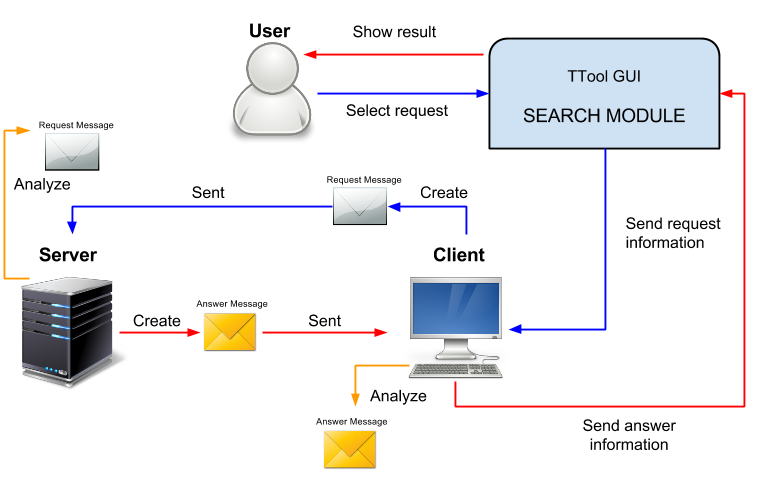
\includegraphics[scale=0.5]{Protocol5.png}\par
	\end{center}
			
	\end {itemize}
	
	\subsection{Implementation}
		\subsubsection{Message}
			\paragraph{Objective} Message is a unified structure between clients and server which supplies useful functions in order to exchange information between them.
			\paragraph{Syntax}
			\begin{itemize} 
\begin{table}[h]
\begin{tabular}{|c|l|c|ll}
\cline{1-3}
\textbf{Parameters} & \textbf{Description} & \textbf{Type} &  &  \\ \cline{1-3}
cmd & \begin{tabular}[c]{@{}l@{}}Used for both client and server, to tell which type of message is.\\ From client side, it could be a request message for searching, \\ details, and statistic. From server side, it could be an answer \\ message for searching, details and statistic.\end{tabular} & String &  &  \\ \cline{1-3}
content & \begin{tabular}[c]{@{}l@{}}Used for server to store results in order to send back to clients. \\ It can be a string of xml, a byte array for transferring an image\end{tabular} & \begin{tabular}[c]{@{}c@{}}ArrayList\\ \textless Object\textgreater\end{tabular} &  &  \\ \cline{1-3}
options & \begin{tabular}[c]{@{}l@{}}Used for client side only. It will contain the name of all values\\ in the \textit{values} variable. The order of values in \textit{options} will follow:\\\textbf{Keyword - Year - System - Score - NumberOfRecord} \end{tabular} & \begin{tabular}[c]{@{}c@{}}ArrayList\\ \textless Object\textgreater\end{tabular} &  &  \\ \cline{1-3}
values & \begin{tabular}[c]{@{}l@{}}Used for client side to store all the real data respectively with \\values in \textit{options}. \end{tabular} & \begin{tabular}[c]{@{}c@{}}ArrayList\\ \textless Object\textgreater\end{tabular} &  &  \\ \cline{1-3}

\end{tabular}
\caption{Variables of a message}
\label{table:messVariable}
\end{table}
			\item The used variables of a message is described in Table \ref{table:messVariable}
			\item Both options and values are ArrayList$\textless$String$\textgreater$ type and used for clients to let the server know what information the user wants to retrieve. for options, it could be an arraylist of string which contains strings both clients and server unified before. Beside that, values represents for real values respectively along with options. Take a look at one example for options and values in Table \ref{table:opvaex}
			
\begin{table}[h]
\centering
\begin{tabular}{|c|c|c|c|c|c|}
\hline
\textbf{\textless options\textgreater} & Keyword & Year & System & Score & NumberOfRecord \\ \hline
\textbf{\textless values\textgreater} & Buffer-overflow & Last year & Linux & 7-8 & 10 \\ \hline
\end{tabular}
\caption{An example of how to assign options and values}
\label{table:opvaex}
\end{table}


\begin{table}[h]
\centering
\begin{tabular}{|c|l|c|}
\hline
{\bf Function} & {\bf Description} & {\bf Returned Type} \\ \hline
addOptionValueMessage & \begin{tabular}[c]{@{}l@{}}Add an element for both \\ options and values lists\end{tabular} & void \\ \hline
addKeywordMessage & \begin{tabular}[c]{@{}l@{}}Add an element into values list\\  with "keyword" to option list\end{tabular} & void \\ \hline
createRequestMessage & \begin{tabular}[c]{@{}l@{}}Create a request message \\ from client\end{tabular} & void \\ \hline
createAnswerMessage & \begin{tabular}[c]{@{}l@{}}Create an answer message\\  from server\end{tabular} & void \\ \hline
convertImageToByte & \begin{tabular}[c]{@{}l@{}}Used by server to convert \\ an image to a byte array\end{tabular} & byte{[}{]} \\ \hline
convertByteToImage & \begin{tabular}[c]{@{}l@{}}Used by clients to convert \\ a byte array to an image\end{tabular} & void \\ \hline
\end{tabular}
\caption{Functions of Message}
\label{table:functionsMessage}
\end{table}



\paragraph{Message Types}
	\begin{itemize}[label={$\circ$}]
		\item Search message structure is described in Table \ref{search}
		\item Detail message structure is described in Table \ref{detail}
		\item Statistics message structure is described in Table \ref{stat}
		\item Histogram message structure is described in Table \ref{histogram}
		
\paragraph{Implementation}
		The source code is implemented in file \textit{./src/myutils/externalSearch/Message.java} \ref{table:functionsMessage}
		
	\end{itemize}
	 \begin{table}[h]
\centering
\begin{tabular}{|c|l|l|l|l|l|l|l|l|l|l|l|}
\hline
\multicolumn{6}{|c|}{{\bf CLIENT}}                         & \multicolumn{6}{c|}{{\bf SERVER}}                                                                   \\ \hline
{\bf cmd}     & \multicolumn{5}{l|}{Search}                & \multicolumn{6}{l|}{SearchResult}                                                                   \\ \hline
{\bf content} & \multicolumn{5}{l|}{}                      & \multicolumn{6}{l|}{\begin{tabular}[c]{@{}l@{}}Result from the server\\ in XML format\end{tabular}} \\ \hline
{\bf options} & Keyword & Year      & System & Score & NoR & \multicolumn{6}{l|}{}                                                                               \\ \hline
{\bf values}  & Stuxnet & This year & Linux  & 7-8   & 10  & \multicolumn{6}{l|}{}                                                                               \\ \hline
\end{tabular}
\caption{Structure of Search message and SearchResult message}
\label{search}
\end{table}
		
		\begin{table}[h]
\centering
\begin{tabular}{|c|l|l|l|l|l|l|l|l|l|l|l|}
\hline
\multicolumn{6}{|c|}{{\bf CLIENT}}            & \multicolumn{6}{c|}{{\bf SERVER}}  \\ \hline
{\bf cmd}      & \multicolumn{5}{l|}{Detail}  & \multicolumn{6}{l|}{DetailResult}  \\ \hline
{\bf content}  & \multicolumn{5}{l|}{}        & \multicolumn{6}{l|}{Result  from the server in XML format} \\ \hline
{\bf options}  & \multicolumn{5}{l|}{Keyword} & \multicolumn{6}{l|}{}              \\ \hline
{\bf values}   & \multicolumn{5}{l|}{CVE ID}  & \multicolumn{6}{l|}{}              \\ \hline
\end{tabular}
\caption{Structute of Detail message and DetailResult message}
\label{detail}
\end{table}
\begin{table}[h]
\centering
\begin{tabular}{|c|l|l|l|l|l|l|l|l|l|l|l|}
\hline
\multicolumn{6}{|c|}{{\bf CLIENT}}                                                                                                          & \multicolumn{6}{c|}{{\bf SERVER}}  \\ \hline
{\bf cmd}      & \multicolumn{5}{l|}{Stat}                                                                                                  & \multicolumn{6}{l|}{StatResult}  \\ \hline
{\bf content}  & \multicolumn{5}{l|}{}                                                                                                      & \multicolumn{6}{l|}{Binary String} \\ \hline
{\bf options}  & \multicolumn{5}{l|}{Keyword}                                                                                               & \multicolumn{6}{l|}{}              \\ \hline
{\bf values}   & \multicolumn{5}{l|}{\begin{tabular}[c]{@{}l@{}}This can be several keyword in a string\\ "Linux Sql Windows"\end{tabular}} & \multicolumn{6}{l|}{}              \\ \hline
\end{tabular}
\caption{Structure of Statistics message and ResultStatistics message}
\label{stat}
\end{table}
\begin{table}[h]
\centering
\begin{tabular}{|c|l|l|l|l|l|l|l|l|l|l|l|}
\hline
\multicolumn{6}{|c|}{{\bf CLIENT}}                                                                   & \multicolumn{6}{c|}{{\bf SERVER}}  \\ \hline
{\bf cmd}      & \multicolumn{5}{l|}{Histogram}                                                           & \multicolumn{6}{l|}{HistogramResult}  \\ \hline
{\bf content}  & \multicolumn{5}{l|}{}                                                               & \multicolumn{6}{l|}{Binary String} \\ \hline
{\bf options}  & \multicolumn{5}{l|}{Keyword}                                                        & \multicolumn{6}{l|}{}              \\ \hline
{\bf values}   & \multicolumn{5}{l|}{\begin{tabular}[c]{@{}l@{}}One key word\\ "Linux"\end{tabular}} & \multicolumn{6}{l|}{}              \\ \hline
\end{tabular}
\caption{Structure of Histogram message and HistogramResult message}
\label{histogram}
\end{table}		
\end{itemize}		
\subsubsection{Client}
			\paragraph{Objective} 
			Receive request information from the Search Module, then create a request and send to server. Then, client analyze an answer message from server. Depends on which type of the answer message, client will call right functions to interact with users via TTool GUI. In specific, the type of the answer message is stored in the variable “cmd” (command), if command is result for search or detail, client will read and show information via the Database tab. If the command is result for details, it will show an image.
\paragraph{Implementation} 
		Related source code relating to Client in TTool:
		\begin{itemize}[label={$\circ$}]
		\item ./src/myutils/externalSearch/Client.java \ref{table:functionsClient}
		\item ./src/myutils/externalSearch/Record.java : Used to parse the content of return messages 				
\end{itemize}
\begin{table}[h]
\centering
\begin{tabular}{|c|l|c|}
\hline
{\bf Function}      & \multicolumn{1}{c|}{{\bf Description}}                                                                          & {\bf Returned Type} \\ \hline
parserAnswerMessage & \begin{tabular}[c]{@{}l@{}}Parse the message from the server \\ depends on the type of the message\end{tabular} & Object              \\ \hline
send                & \begin{tabular}[c]{@{}l@{}}Send a message to the server via \\ SSL Socket and waits for response\end{tabular}   & Message             \\ \hline
\end{tabular}
\caption{Functions of Client}
\label{table:functionsClient}
\end{table}
\subsubsection{Server}
\paragraph{Objective} 
Server receives requests from the client through a request message, then it will analyze and search for relevant information. Finally, it will extract all information as an answer message and send back to the client. 
\paragraph{Implementation} 
Related source code relating to Server in Crawler \textit{./src/web/crawler/MultiThreadSerer.java} \ref{table:functionsServer}
\begin{table}[h]
\begin{tabular}{|c|l|c|}
\hline
\textbf{Function} & \textbf{Description} & \textbf{Type} \\ \hline
analyseRequestMessage & Analyze the request message sent from the server & void \\ \hline
createAnswerMessage & \begin{tabular}[c]{@{}l@{}}Create an answer message with relevant information\\ from searching or databases\end{tabular} & Message \\ \hline
\end{tabular}
\caption{Functions of Server}
\label{table:functionsServer}
\end{table}
	
\mychapter{5}{Conclusion}
In summary, we successfully succeeded in describing Stuxnet attack by a SysML-Sec model. In addition, we designed a friendly user interface which allows users interact with databases for retrieving relevant information. Finally, we also implemented a protocol for exchanging messages between users and the web crawler database.

\begin{bibdiv}
\begin{biblist}
\bibselect{references}
\end{biblist}
\end{bibdiv}
\end{document}